%++++++++++++++++++++++++++++++++++++++++
% Don't modify this section unless you know what you're doing!
\documentclass[a4paper,12pt]{article}
\usepackage{listings} % code blocks
\usepackage{tabularx} % extra features for tabular environment
\usepackage{amsmath}  % improve math presentation
\usepackage{graphicx} % takes care of graphic including machinery
\usepackage{subcaption} % necessary for subfigures
\usepackage{float}
\usepackage[margin=3.0cm,a4paper]{geometry} % decreases margins
%\usepackage{cite} % takes care of citations
%\usepackage[final]{hyperref} % adds hyper links inside the generated pdf file
%++++++++++++++++++++++++++++++++++++++++

\setlength{\parindent}{0pt}
\usepackage{hyperref}

\begin{document}

\title{Deep Learning Lab \\ Exercise 04 }
\author{Rabea Turon \& Megan Klaiber}
\date{\today}
\maketitle

\section{Introduction}

In this exercise a DQN agent will be implemented and its prformance willl be evaluated on the CartPole and CarRacing environment of OpenAI Gym.


\section{Reinforcement Learning: Deep Q-Networks}\label{rl}


\subsection{CartPole}\label{cartpole}

A simple neural network was used for the CartPole task. It consists of two fully connected layers each with 20 hidden units. The network is optimized with mean squared error and Adam optimizer. CartPole is considered solved when the average reward is greater than or equal to 195.0 over 100 consecutive episodes. So we stopped the training when this point was reached. The size of the batches sampled from the replay buffer was 64 and we used a learning rate of 0.001.\\

\autoref{fig:cartpole_episode_reward} shows the achieved reward during the training episodes. Here CartPole was solved after 150 episodes. During training every 20th episode the agent was evaluated with deterministic actions over 5 episodes. The average reward of these 5 episodes is shown in \autoref{fig:cartpole_evaluation_reward}. The final performance where evaluated over 15 test episodes. Here the average reward was 349 with a standard deviation of 72.


\begin{figure}[H]
	\centering 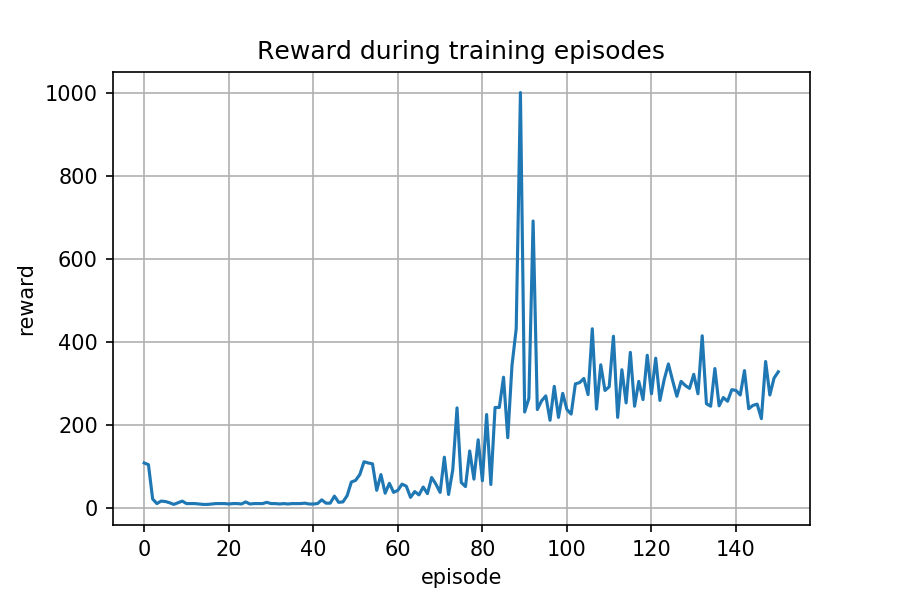
\includegraphics[width=11.70cm, height=7.9cm]{plots/cartpole_episode_reward.png}
	\caption{
		\label{fig:cartpole_episode_reward}
		Achieved reward during training episodes.
	}
\end{figure}

\begin{figure}[H]
	\centering 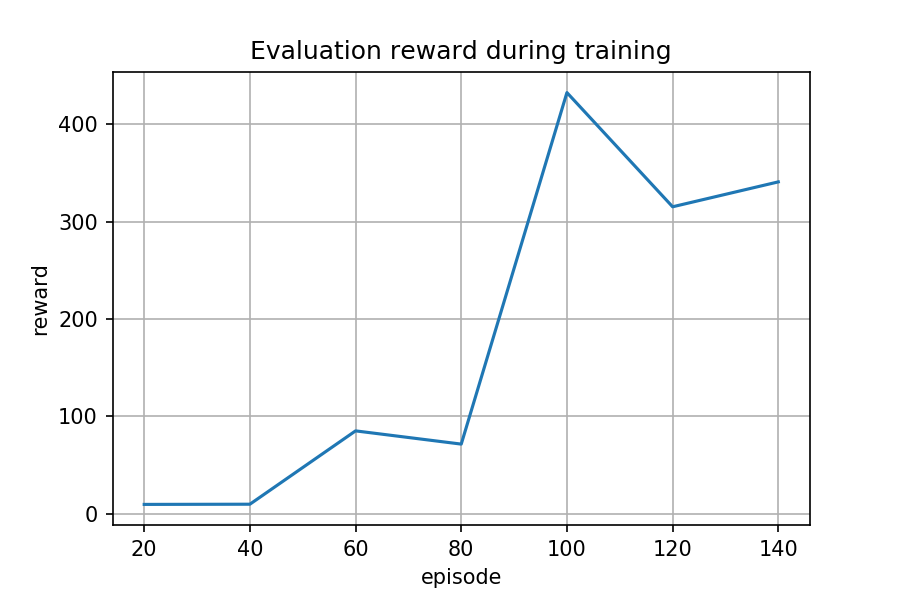
\includegraphics[width=11.70cm, height=7.9cm]{plots/cartpole_evaluation_reward.png}
	\caption{
		\label{fig:cartpole_evaluation_reward}
		Evaluated agent with deterministic actions every 20th episodes (mean episode reward over 5 episodes).
	}
\end{figure}

\subsection{CarRacing}\label{carracing}

%\begin{figure}[H]
%	\centering 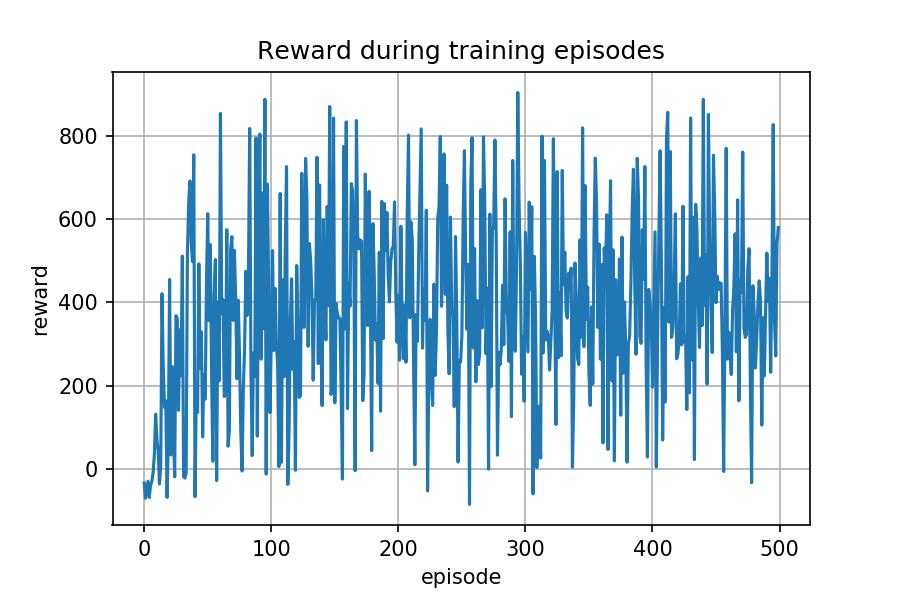
\includegraphics[width=11.70cm, height=7.9cm]{plots/carracing_episode_reward.png}
%	\caption{
%		\label{fig:carracing_episode_reward}
%		Achieved reward during training episodes.
%	}
%\end{figure}

%\begin{figure}[H]
%	\centering 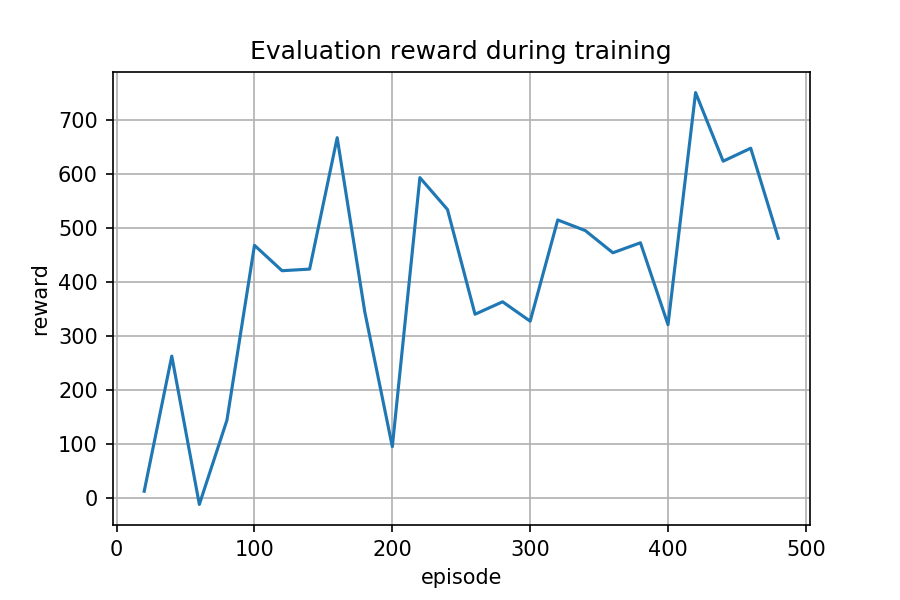
\includegraphics[width=11.70cm, height=7.9cm]{plots/carracing_evaluation_reward.png}
%	\caption{
%		\label{fig:carracing_evaluation_reward}
%		Evaluated agent with deterministic actions every 20th episodes (mean episode reward over 5 episodes).
%	}
%\end{figure}

\section{Conclusion}



\end{document}
